\documentclass{article}
\usepackage[utf8]{inputenc}
\usepackage{geometry}
 \geometry{
 a4paper,
 total={170mm,257mm},
 left=20mm,
 top=20mm,
 }
 \usepackage{graphicx}
\usepackage{titling}
\usepackage{hyperref}
\usepackage{xcolor}

\title{Card Counting Blackjack: Phase 2}
\date{30/6/2025}

 
 \usepackage{fancyhdr}
\fancypagestyle{plain}{%  the preset of fancyhdr 
    \fancyhf{} % clear all header and footer fields
    \fancyhead[L]{Reinforcement Learning and Dynamic Optimization}
    \fancyhead[R]{\thedate}
    \fancyfoot[C]{\thepage}
}
\makeatletter
\def\@maketitle{%
  \newpage
  \null
  \vskip 1em%
  \begin{center}%
  \let \footnote \thanks
    {\LARGE \@title \par}%
    \vskip 1em%
    %{\large \@date}%
  \end{center}%
  \par
  \vskip 1em}
\makeatother

\usepackage{lipsum}
\usepackage{amsmath}
\usepackage{cmbright}

\begin{document}

\maketitle

\noindent\begin{tabular}{@{}ll}
     Michalis Lamprakis & 2020030077\\
     Dimitris Ilia & 2020030200
\end{tabular}

\section*{Project context}

The goal of the second phase of the project is to make a more realistic
Blackjack environment and hopefully "beat" the casino. The environment
now inludes betting option, double down action and 3/2 payout in natural 
blackjack. The project is structured in 2 subtasks: i) fixed 1\$ bet
at the start of each round and ii) agent to chooses the initial bet. 

\section*{Implementantion}
The whole implementantion is based on {\bf BlackjackEnv} class that
we made from scratch ,with the help of online tools and resources,
and contains all the necessary methods to simulate the game.
The provided code contains detailed comments.\\\\
{\bf Task 1}\\
In this task, there is a fixed bet of 1\$ at the start of each round with
the option to double down. Natural blackjack pays 1.5 times the bet.
We train an agent to find the optimal policy (with and without Card Counting) 
using tabular Q-learning
and Bellman equation.
\[
  Q(s, a) \leftarrow Q(s, a) + \alpha \left( r + \gamma \max_{a'} Q(s', a') - Q(s, a) \right)
\]

\noindent The state space consists of 
\begin{itemize}
  \item \((\text{player's total}, \text{dealer's upcard}, \text{usable ace}, \text{can\_double})\) for the basic agent
  \item  \((\text{player's total}, \text{dealer's upcard}, \text{usable ace}, \text{can\_double}, \text{hi\_lo\_bucket})\) for the hi-lo environment
\end{itemize}

\noindent {\bf can\_double} is a boolean indicating whether the player can double down.\\\\
After experimenting with different parameters, we decided to use
\begin{itemize}
  \item {\bf Alpha}: decayed linearly from 0.1 to 0.01 across 200,000 episodes
  \item {\bf Gamma}: 1.0
  \item {\bf Epsilon}: decayed linearly from 1 to 0.05 across 1M episodes
\end{itemize}

\noindent The agent is trained for 5M episodes (for both cases) and evaluated
for 100K episodes with the learned policy, we capture the following results:
\begin{table}[h!]
\centering
\begin{tabular}{|l|c|c|}
\hline
 & \textbf{Basic Agent} & \textbf{Hi-Lo Agent} \\
\hline
{\bf Average profit per game} & {\bf -0.02\$} & {\bf -0.01\$} \\
Average bet size & 1.00\$ & 1.00\$ \\
Double-down rate & 1.36\% & 2.37\% \\
Double-down win rate & 64.75\% & 59.53\% \\
Win & 43.25\% & 43.74\% \\
Draw & 9.13\% & 8.72\% \\
Lose & 47.62\% & 47.55\% \\
\hline
\end{tabular}
\end{table}

\noindent We observe that the hi-lo agent performs better than the basic agent,
which is expected as it uses card counting to adjust its strategy, but still
both agents have a negative average profit per game. Also the hi-lo is
more confident to double down, as it has more information about the remaining cards.

\newpage

\begin{figure}[h!]
  \centering
  \begin{minipage}{0.48\textwidth}
    \centering
    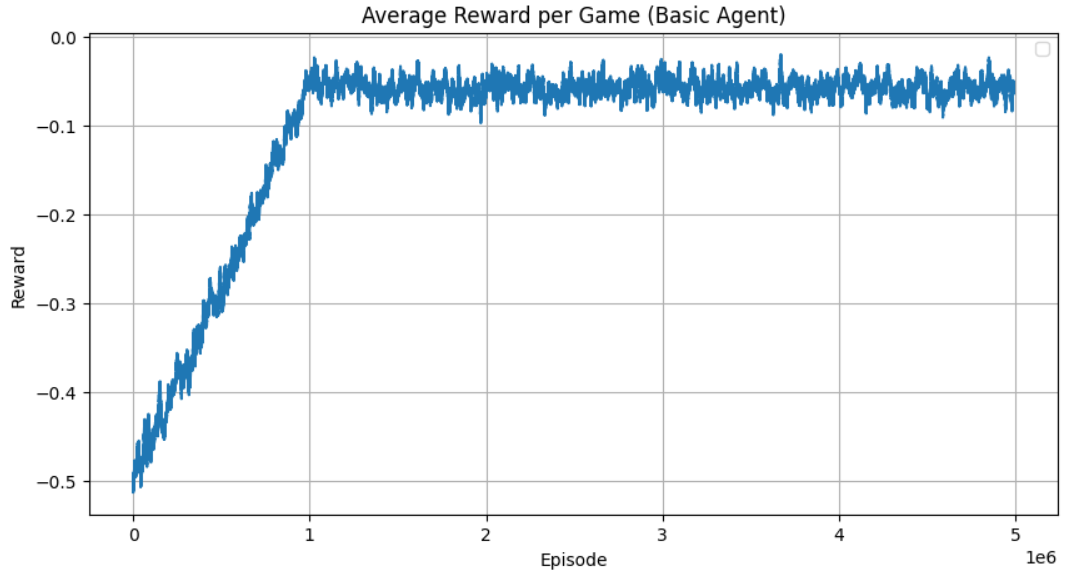
\includegraphics[width=\linewidth]{Images/rew_basic.png}
    \label{fig:basic_agent_profit}
  \end{minipage}\hfill
  \begin{minipage}{0.48\textwidth}
    \centering
    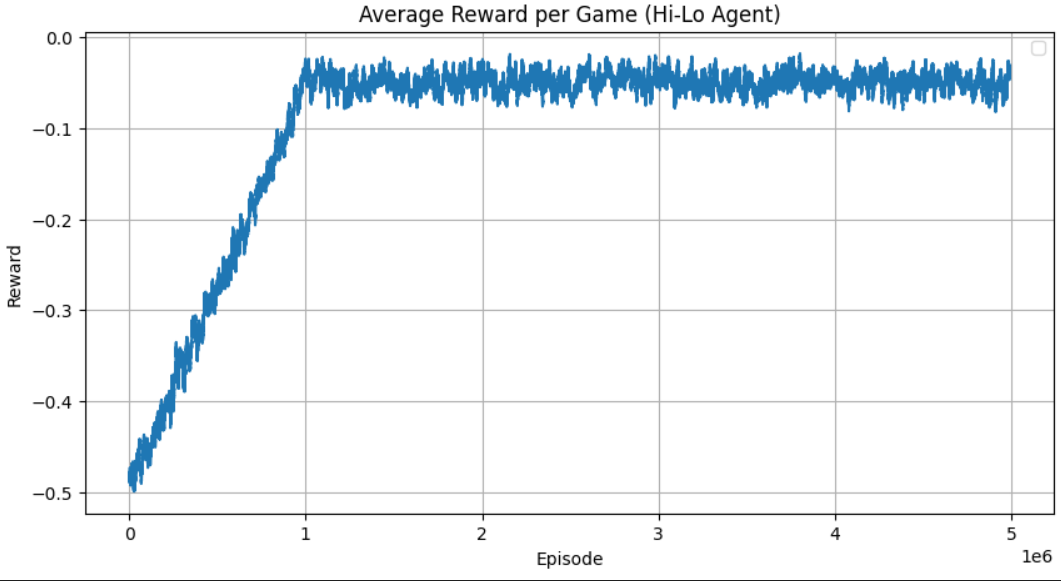
\includegraphics[width=\linewidth]{Images/rew_hilo.png}
    \label{fig:hilo_agent_profit}
  \end{minipage}
  \caption{Average reward per episode for the Basic Agent (left) and Hi-Lo Agent (right).}
\end{figure}

\noindent To monitor the learning progress of our Q-learning agent, 
we tracked the average reward per episode throughout training.
At the beginning of training, the agent explores heavily, 
resulting in highly variable returns. 
As training progresses and the exploration rate decays, 
the agent converges to a more stable policy.\\\\

\noindent We also did the comparison of our learned policy with the 
proven best strategy for Blackjack and we observed 96-97\%
compliance which is a proof that our agent has learned the optimal policy.\\\\

\noindent {\bf Execution details}\\
\noindent For this task there is a menu with the following options:
\begin{itemize}
  \item {\bf 1}: Play manually against the dealer
  \item {\bf 2}: Train the basic Q-agent
  \item {\bf 3}: Evaluate the basic agent
  \item {\bf 4}: Compare the learned policy with the proven best strategy
  \item {\bf 5}: Train the hi-lo agent
  \item {\bf 6}: Evaluate the hi-lo agent
  \item {\bf 7}: Exit
\end{itemize}


\noindent {\bf Task 2}\\
For the second task, we can now choose the bet size at the start of each round.
We implemented two separate neural networks with different roles and 
inputs: a Play Network (DQN) responsible for decision-making during 
gameplay, and a Bet Network (BetNet) responsible for determining 
optimal bet sizes based on card count.\\\\

\noindent The {\bf Play Network} is a Deep Q-Network (DQN) that approximates the optimal 
action-value function 
$Q(s,a)$ for the Blackjack play policy. It learns to choose between Hit, 
Stick, or Double Down, based on the current game state. It is a 
fully connected neural network with 2 hidden layers, 
the first one contains 128 neurons and the second 64.
Both, use ReLU activation.
\begin{itemize}
  \item {\bf Input}: player's total, dealer's upcard, usable ace, can\_double , true count (state vector of size 5)
  \item {\bf Output}: Q-values for HIT (0), STICK (1), DOUBLE (2)
\end{itemize}

\newpage

\noindent We have chosen the following hyperparameters for the DQN:
\begin{itemize}
  \item {\bf Alpha}: 1e-4 
  \item {\bf Gamma}: 1.0
  \item {\bf Epsilon}: decayed linearly from 1.0 to 0.05 across 1M episodes
  \item {\bf Batch Size}: 128
  \item {\bf Replay Buffer Size}: 200,000 transitions
  \item {\bf Target Network Update Frequency}: every 5,000 steps
\end{itemize}

\vspace{1em}

\noindent The {\bf BetNet} is a separate neural network that learns a bet sizing policy 
based only on the true count.
It outputs a Distribution over 10 discrete bet sizes (\$1–\$10) ,allowing 
the agent to bet more when the deck is favorable and less when it is not.
It is also a smaller fully connected neural network with 2 hidden layers,
the first one contains 64 neurons and the second 32. 
The activation function is ReLU for both layers.
\begin{itemize}
  \item {\bf Input}: true count (state vector of size 1)
  \item {\bf Output}: Distribution over bet sizes (10 outputs)
\end{itemize}

\noindent And the hyperparameters for the BetNet:
\begin{itemize}
  \item {\bf Alpha}: 1e-4 
  \item {\bf Gamma}: 1.0
  \item {\bf Epsilon}: decayed linearly from 1.0 to 0.05 across 1M episodes
  \item {\bf Batch Size}: 128
  \item {\bf Replay Buffer Size}: 200,000 transitions
  \item {\bf Target Network Update Frequency}: every 5,000 steps
\end{itemize}

\noindent After training both networks for 1.6M episodes, we evaluate the agent for
another 100K episodes and we capture the following results (for 1 deck
and 4 decks environment):

\begin{table}[h!]
\centering
\begin{tabular}{|l|c|c|}
\hline
 & \textbf{1 Deck} & \textbf{4 Decks} \\
\hline
{\bf Average profit per game} & {\bf 0.09\$} & {\bf 0.04\$} \\
Average bet size & 5.13\$ & 4.15\$ \\
Expected return per unit bet & 0.0182 &  0.0104\\
Double-down rate & 8.79\% & 6.63\% \\
Double-down win rate & 55.73\% & 54.95\% \\
Win & 44.00\% & 43.48\% \\
Draw & 8.27\% & 8.81\% \\
Lose & 47.73\% & 47.71\% \\
\hline
\end{tabular}
\end{table}

\noindent We observe that the agent performs significantly better than the previous
task, achieving a positive average profit per game, which means the agent is 
statistically profitable and effectively beating the casino under these settings.
\noindent The agent is more confident to double down, as it has more information
about the remaining cards and it can adjust its bet size according to them.
Without the betting network, the DQN policy would be almost the same as Task1.
So the key innovation here is the BetNet, which allows the agent to adjust its bet size based on the true count.
This means the agent bets more when the deck is favorable, just like a real card counter.
We can see exaclty this in {\bf Figure 2}. Agent maximizes its bet size when the true count is high,
and minimizes it when the true count is low. This is a clear indication that the agent has learned to use card counting effectively to adjust its betting strategy.

\newpage

\begin{figure}[h!]
  \centering
  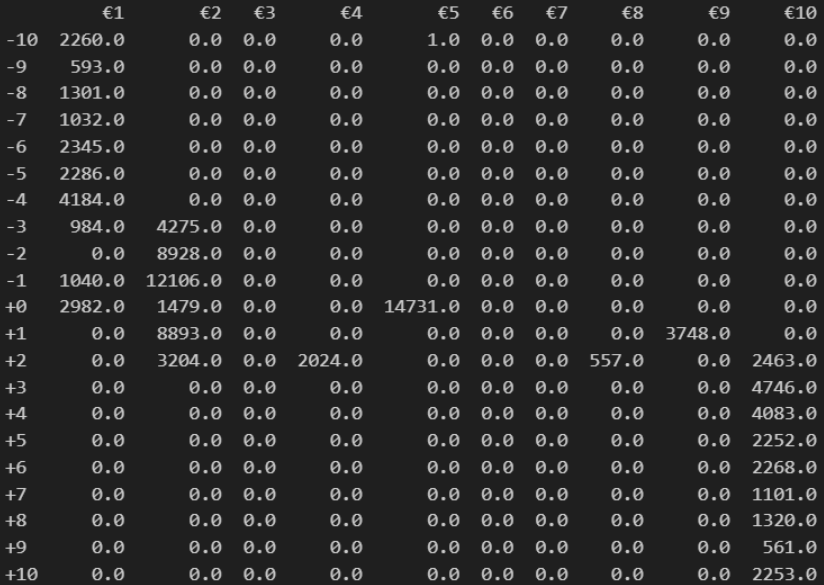
\includegraphics[width=0.7\linewidth]{Images/bettable.png}
  \caption{BetNet's distribution over bet sizes for different true counts.}
  \label{fig:betnet_distribution}
\end{figure}

\noindent The following plot (left) shows the moving average reward per episode
 during the training of the DQN play policy. Initially,
  the agent performs poorly. As training 
  progresses, the average reward steadily improves and 
  stabilizes, reflecting the agent's convergence 
  toward a near-optimal policy. The right plot shows the 
  TD-loss over time that steadily decreases during 
  training, indicating improved accuracy in the agent's
   Q-value predictions. 

\begin{figure}[h!]
  \centering
  \begin{minipage}{0.48\textwidth}
    \centering
    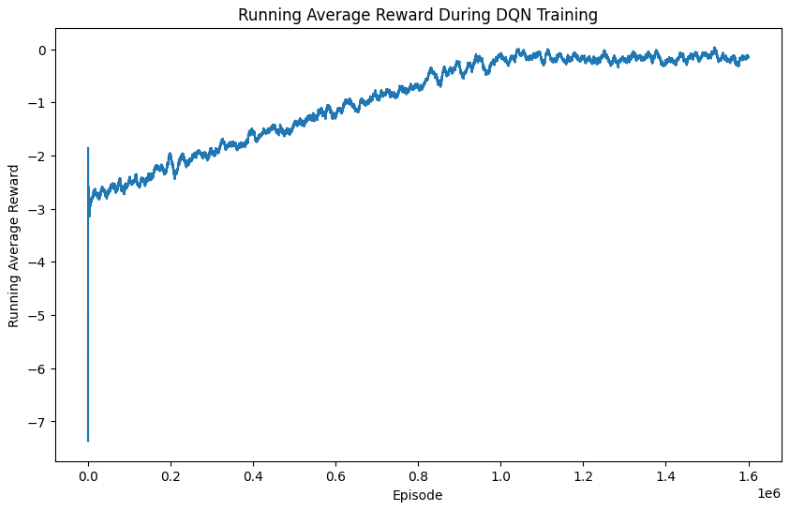
\includegraphics[width=\linewidth]{Images/dqn_reward.png}
    \label{fig:left_plot}
  \end{minipage}\hfill
  \begin{minipage}{0.48\textwidth}
    \centering
    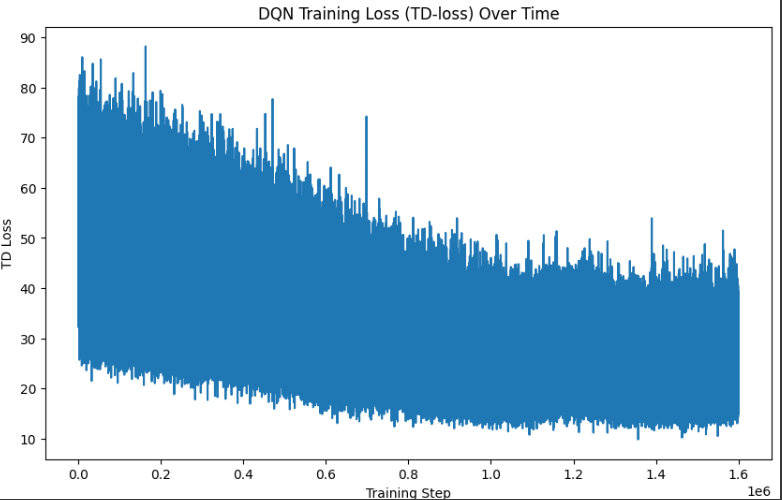
\includegraphics[width=\linewidth]{Images/td_;oss.png}
    \label{fig:right_plot}
  \end{minipage}
  \caption{Average reward for the DQN agent (left) and the TD-loss over time (right).}
\end{figure}


\noindent {\bf Execution details}\\
\noindent Menu options:
\begin{itemize}
  \item {\bf 1}: Train DQN agent with BetNet
  \item {\bf 2}: Evaluate 
  \item {\bf 3}: Compute confidence interval
  \item {\bf 4}: load NNs and evaluate (in case we save our models)
  \item {\bf 5}: Exit
\end{itemize}

\noindent All the above are implemented in {\bf PHASE\_2.ipynb file}.\\\\

\newpage

\noindent {\bf Conclusion}\\
With this project we have successfully implemented a realistic Blackjack environment
and trained agents that can play the game effectively. Started in Phase 1 with a basic
agent achieving a negative average reward of {\bf-0.06\$} per game
and ended up in Phase 2 with an "advantage" agent that can adjust its betting strategy
and achieve a positive average reward up to {\bf 0.09\$} per game which is
pretty impressive.\\\\


\noindent {\bf Notes}\\
In phase 1 while at first we used a learning rate of 0.1, as you told us and
then we found out ourselves, it was too high and it caused unstability in the training process,
so we decided to use 0.01. As we can see in the following plots,
the average reward stabilizes and also we tracked agent’s chosen action evolved for 
three high-impact states:
\begin{itemize}
  \item (18,10,0)
  \item (13,5,0)
  \item (15,10,0)
\end{itemize}
\noindent The agent initially fluctuated but converged.

\begin{figure}[h!]
  \centering
  \begin{minipage}{0.48\textwidth}
    \centering
    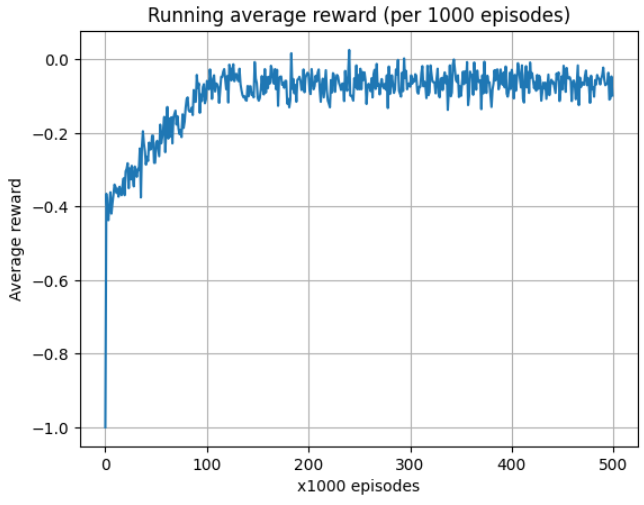
\includegraphics[width=\linewidth]{Images/0.01a_plot.png}
    \label{fig:0.01a_plot}
  \end{minipage}\hfill
  \begin{minipage}{0.48\textwidth}
    \centering
    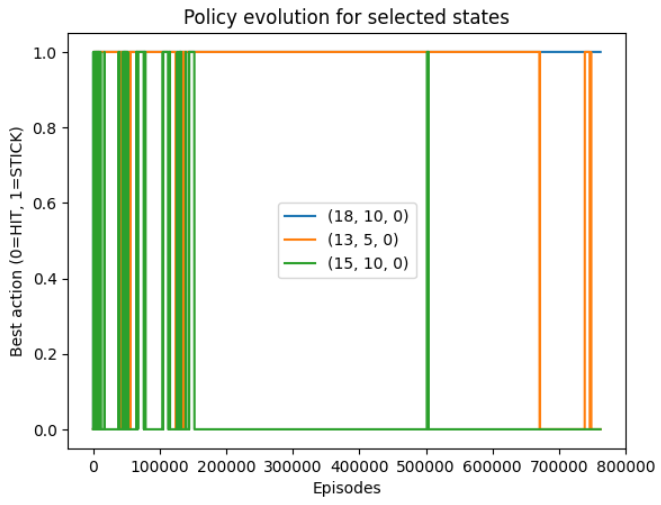
\includegraphics[width=\linewidth]{Images/0.01a_plot.2.png}
    \label{fig:0.01a_plot_2}
  \end{minipage}
  \caption{Average reward per episode for the Basic Agent with learning rate 0.01 (left) and the agent's chosen actions for three high-impact states (right).}
\end{figure}





\end{document}